\chapter{Neural Optimal Transport with Context}
\label{cha:condot}

\dictum[Stefan Zweig, \textit{Verwirrung der Gef{\"u}hle} (1927)]{%
  Auch die Pause geh{\"o}rt zur Musik.}%
\vskip 2em

\verpar{Contributions}{
Most of the material in this chapter has been already published in the following conference proceedings:
\begin{itemize}
	\item[] Charlotte Bunne, Andreas Krause, and Marco Cuturi. Supervised Training of Conditional Monge Maps. In \textit{Advances in Neural Information Processing Systems (NeurIPS)}, 2022.
	\vspace{-9pt}
\end{itemize}
}

A key challenge in the treatment of cancer is to predict the effect of drugs, or a combination thereof, on the cells of a particular patient. To achieve that goal, single-cell sequencing can now provide measurements for individual cells, in treated and untreated conditions, but these are, however, not in correspondence.  Given such examples of untreated and treated cells under different drugs, can we predict the effect of new drug combinations?  We develop a general approach motivated by this and related problems, through the lens of optimal transport theory, and, in that process, develop tools that might be of interest to other application domains of OT. Given a collection of $N$ pairs of measures $(\mu_i,\nu_i)$ over $\R^d$ (cell measurements), tagged with a context $c_i$ (encoding the treatment), we seek to learn a context-dependent, parameterized transport map $\mathcal{T}_{\theta}$ such that, on training data, that map $\mathcal{T}_{\theta}(c_i):\mathbb{R}^d\rightarrow\mathbb{R}^d$ fits the dataset, in the sense that $\mathcal{T}_{\theta}(c_i) \sharp\mu_i \approx \nu_i$. Additionally, we expect that this parameterized map can generalize to unseen contexts and patients, to predict, given a patient's cells described in $\mu_{\text{new}}$, the effect of applying context $c_{\text{new}}$ on these cells as $\mathcal{T}_{\theta}(c_{\text{new}})\sharp\mu$. \\

In this chapter, we introduce a framework that can leverage \textit{labeled} pairs of measures $\{(\cont_i, (\mu_i, \nu_i))\}_i$ to infer a \textit{global} parameterized map $\mathcal{T}_{\theta}$. 
% For each observation one has that $\mu_i,\nu_i\in\mathcal{P}(\mathbb{R}^d)$ is a pair of probability measures, while 
Hereby, the context $\cont_i$ belongs to an arbitrary set $\mathcal{C}$. We construct $\mathcal{T}_{\theta}$ so that it should be able, given a possibly unseen context label $\cont\in\gC$, to output a map $\mathcal{T}_{\theta}(c):\mathbb{R}^d\rightarrow\mathbb{R}^d$, that is itself the gradient of a convex function. To that end, we propose to learn these parameterized Monge maps $\mathcal{T}_{\theta}$ as the gradients of \acrshortpl{PICNN}, which we borrow from the foundational work of \citet{amos2017input}. 

\looseness -1 \cref{cha:cellot} exploited an explicit connection between OT and neural networks derived from the celebrated \citeauthor{brenier1987decomposition} theorem \citeyearpar{brenier1987decomposition}.
In this chapter, we build on this line of work, but substantially generalize it, to learn a {\em parametric} family of context-aware transport maps, using a collection of labeled pairs of measures.
Our framework can be also interpreted as a hypernetwork \citep{ha2016hypernetworks}: The \acrshort{PICNN} architecture can be seen as an \acrshort{ICNN} whose weights and biases are \textit{modulated} by the context vector $\cont$, which parameterizes a \textit{family} of convex potentials in $\mathbb{R}^d$.
%
Because both \acrshortpl{ICNN} ---and to a greater extent \acrshortpl{PICNN}--- are notoriously difficult to train~\citep{richter2021input,korotin2021wasserstein,korotin2021neural}, we use closed-form solutions between Gaussian approximations to derive relevant parameter initializations for (P)ICNNs:
These choices ensure that \textit{upon initialization}, the gradient of the (P)ICNNs mimics the affine Monge map obtained in closed form between Gaussian approximations of measures $\mu_i,\nu_i$~\citep{gelbrich1990formula}.
%
Our framework is applied to three scenarios: Parameterization of transport through a real variable (time or drug dosage), through an auxiliary informative variable (cell covariates), and through action variables (genetic perturbations in combination) (see \cref{fig:overview_condot}). Our results demonstrate the ability of our architectures to better capture on out-of-sample observations the effects of these variables in various settings, even when considering never-seen, composite context labels. These results suggest potential applications of conditional OT to model personalized medicine outcomes, or to guide novel experiments, where OT could serve as a predictor for never tested context labels.


\begin{figure*}
    \centering
    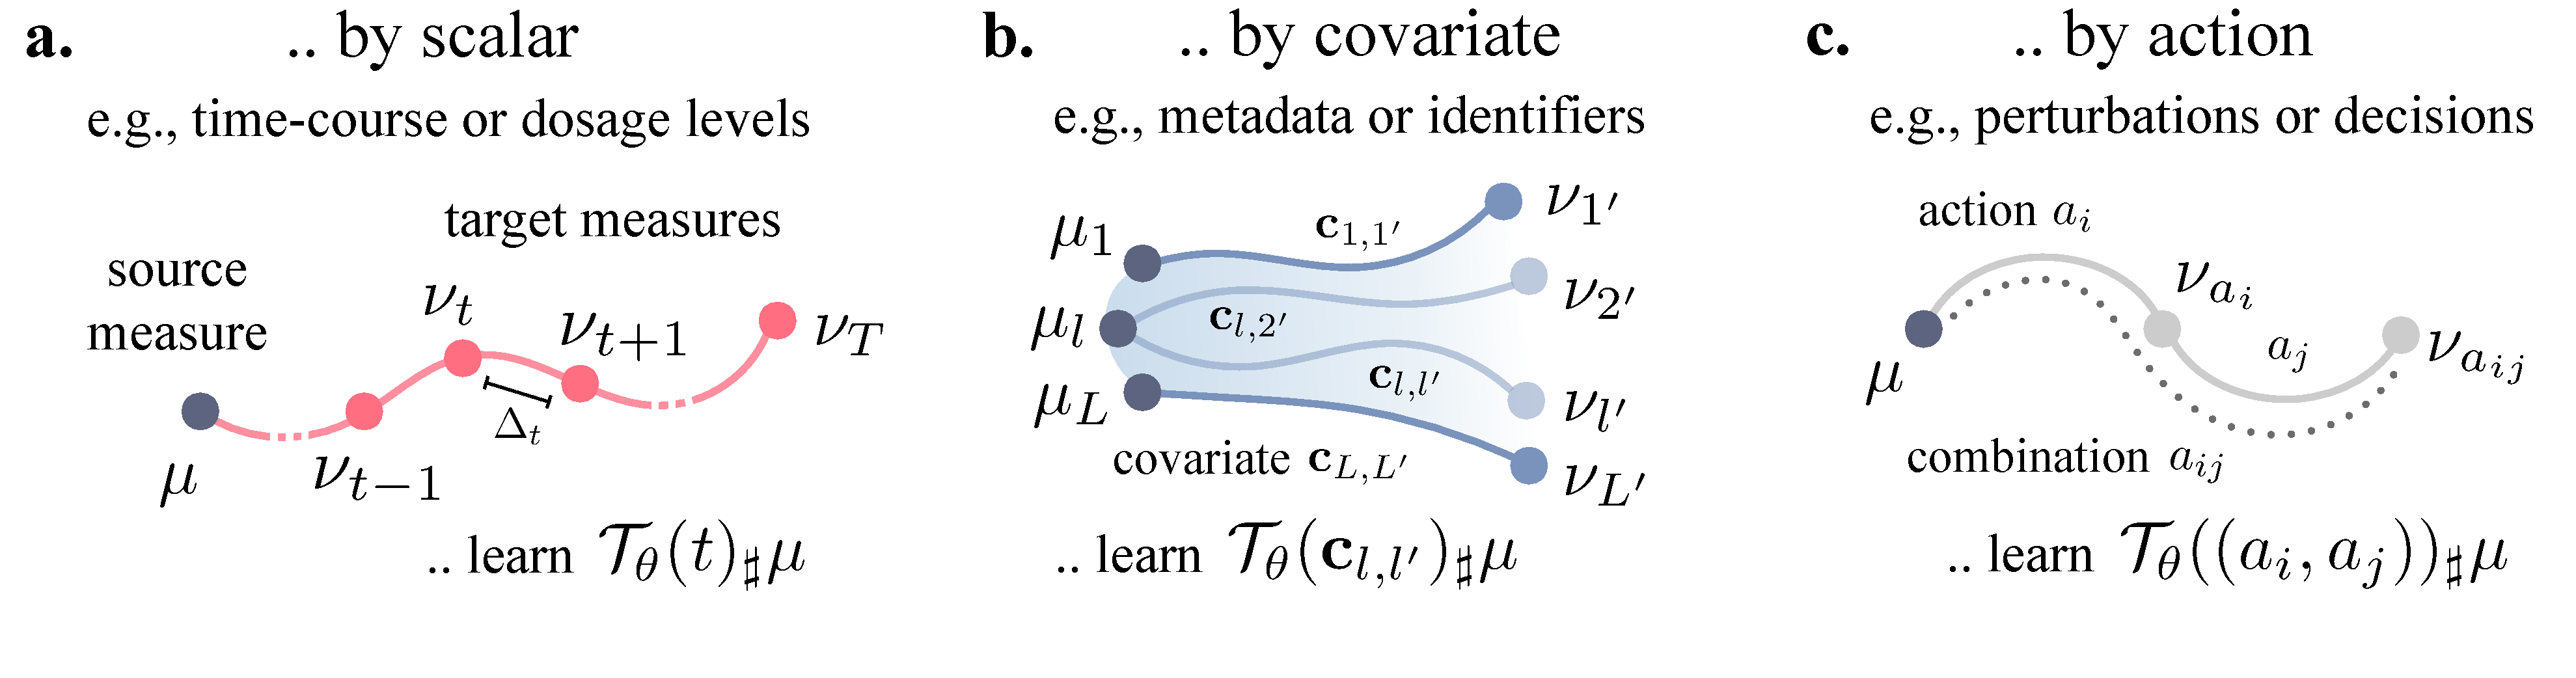
\includegraphics[width= \textwidth]{figures/fig_overview_condot.pdf}
    \caption{The evolution from a source $\mu$ to a target measure $\nu$ can depend on context variables $\cont$ of various nature. This comprises \textbf{a.} scalars such as time or dosage $t$ which determine the magnitude of the optimal transport, \textbf{b.} flow of measures into another one based on additional information (possibly different between $\mu$ and $\nu$) stored in vectors $\mathbf{c}_{l,l^\prime}$, or \textbf{c.} discrete and complex actions $a_i$, possibly in combination $a_{ij}$. We seek a unified framework to produce a map $\mathcal{T}_\theta(\cont)$ from any type of condition $\cont$. \vspace{-15pt}}
    \label{fig:overview_condot}
\end{figure*}


\section{\textsc{CondOT}: Supervised Training of Conditional Monge Maps} \label{sec:method}
We are given a dataset of $N$ pairs of measures, each endowed with a label, $(c_i,(\mu_i, \nu_i))\in\mathcal{C}\times \mathcal{P}(\RR^d)^2$. Our framework builds upon two pillars: (i.) we formulate the hypothesis that an optimal transport $T^\star_i$ (or, equivalently, the gradient of a convex potential $f^\star_i$) explains how measure $\mu_i$ was mapped to $\nu_i$, given context $c_i$; (ii.) we build on the multi-task hypothesis \citep{caruana1997multitask} that all of the $N$ maps $T^\star_i$ between $\mu_i$ and $\nu_i$ share a common set of parameters, that are \textit{modulated} by context information $c_i$. These ideas are summarized in an abstract regression model described below.

\subsection{A Regression Formulation for Conditional OT Estimation}
\looseness -1 $\theta\in\Theta\subset\mathbb{R}^r$, $\mathcal{T}_\theta$ describes a function that takes an input vector $c\in\mathcal{C}$, and outputs a \textit{function} $\mathcal{T}_\theta(c):\mathbb{R}^d\rightarrow\mathbb{R}^d$, as a hypernetwork would~\citep{ha2016hypernetworks}. Assume momentarily that we are given \textit{ground truth} maps $T_i$, that describe the effect of context $c_i$ on any measure, rather only pairs of measures $(\mu_i,\nu_i)$. This is of course a major leap of faith since even recovering an OT map $T^\star$ from two measures is in itself very challenging~\citep{hutter2021minimax,rigollet2022sample,pooladian2021entropic}. If such maps were available, a direct supervised approach to learn a unique $\theta$ could hypothetically involve minimizing a fit function composed of losses between maps
\begin{align}\label{eq:newobj1}
%\textstyle 
\min_\theta \sum_{i=1}^N \int_{\mathbb{R}^d} \|\mathcal{T}_{\theta}(c_i)(x) - T_i(x)\|^2\, \mathrm{d}\mu_i(x)\,.
\end{align}
Unfortunately, such maps $T_i$ are not given, since we are only provided unpaired samples before $\mu_i$ and after $\nu_i$ that map's application.
By \citeauthor{brenier1987decomposition}'s theorem, we know, however, that such an OT map $T^\star_i$ exists, and that it would be necessarily the gradient of a convex potential function that maximizes \eqref{eq:dual-cvx}. As a result, we propose to modify \eqref{eq:newobj1} to (i.) parameterize, for any $c$, the map $\mathcal{T}_\theta(c)$ as the gradient w.r.t. $x$ of a function $f_\theta(x,c):\mathbb{R}^d\times \mathcal{C}\rightarrow \mathbb{R}$ that is convex w.r.t. $x$, namely $\mathcal{T}_\theta(\cont) := x \mapsto \nabla_1 f_\theta(x,\cont)$; (ii.) estimate $\theta$ by maximizing \textit{jointly} the dual objectives~\eqref{eq:dual-cvx} simultaneously for all $N$ pairs of measures, in order to ensure that the maps are close to optimal, to form the aggregate problem
\begin{align}\label{eq:supdual} 
\textstyle \max_\theta \sum_{i=1}^N \mathcal{E}_{\mu_i,\nu_i}(f_{\theta}(\,\cdot\,, c_i)).
\end{align}
We detail in \cref{sec:neural_solvers} how the Legendre transforms that appear in the energy terms $\mathcal{E}_{\mu_i,\nu_i}$ are handled with an auxiliary function.

\subsection{Integrating Context in Convex Architectures}
We propose to incorporate context variables, in order to modulate a family of convex functions $f_{\theta}(x, c)$
using \acrlongpl{PICNN}. \acrshortpl{PICNN} are neural networks that can be evaluated over a pair of inputs $(x,\cont)$, but which are only required to be convex w.r.t.~$x$. Given an input vector $x$ and context vector $\cont$, a ${L}$-layer PICNN is defined as $\varphi_\theta(x, c) = z_{L},$ where, recursively for $0 \leq {l} \leq {L}-1$ one has
\begin{equation} \label{eq:picnn}
\begin{aligned} 
u_{{l}+1} =&\, a^\prime_{l}\left(V_{l} u_{l}+v_{l}\right), \\
z_{{l}+1} =&\, a_{l}\left(W_{l}^{z}\left(z_{l} \circ\left[W_{l}^{z u} u_{l}+b_{l}^{z}\right]_+\right)+\right.
\left.W_{l}^{x}\left(x \circ(W_{l}^{x u} u_{l}+b_{l}^{x})\right)+W_{l}^{u} u_{l}+b_{l}^u\right), \\
\end{aligned}
\end{equation}
where the PICNN is initialized as $u_{0}=\cont, z_0 = \mathbf{0}$, $\circ$ denotes the Hadamard element-wise product, and $a^\prime_{l}$ is any activation function. The parameters of the PICNN are then given by
$$\theta = \{ V_{l}, W_{l}^{z}, W_{l}^{z u}, W_{l}^{x}, W_{l}^{x u} , W_{l}^{u}, v_{l}, b_{l}^{z}, b_{l}^{x}, b_{l}^u \}.$$ 
Similar to ICNNs, the convexity w.r.t. input variable $x$ is guaranteed as long as activation functions $a_i$ are convex and non-decreasing, and the weight matrices $W_{l}^{z}$ have non-negative entries. We parameterize this by storing them as element-wise applications of softplus operations on precursor matrices of the same size, or, alternatively, by regularizing their negative part. Finally, much like ICNNs, all matrices at the ${L}-1$ layer are line vectors, and their biases scalars.

Such networks were proposed by \citet[Eq. 3]{amos2017input} to address a problem that is somewhat symmetric to ours: Their inputs were labeled as $(y, x)$, where $y$ is a label vector, typically much smaller than that of vector $x$. Their PICNN is convex w.r.t.~$y$, in order to easily recover, given a datapoint $x$ (e.g., an image) the best label $y$ that corresponds to $x$ using gradient descent as a subroutine, i.e. $y^\star(x) = \arg\min_y \text{PICNN}_\theta(x,y)$. PICNNs were therefore originally proposed to learn a parameterized, implicit classification layer, amortized over samples, whose motivation rests on the property that it is convex w.r.t. label variable $y$. By contrast, we use PICNNs that are convex w.r.t. data points $x$. In addition to that swap, we do not use the convexity of the PICNN to define an implicit layer (or to carry out gradient descent). Indeed, it does not make sense in our setting to minimize $\varphi_\theta(x,\cont)$ as a function of $x$, since $x$ is an observation. Instead, our proposal rests on the property that $\nabla_1 \varphi_\theta(x,\cont)$ describes a parameterized family of OT maps. We note that PICNNs were considered within the context of OT in \cite[Appendix B]{fan2021scalable}. In that work, PICNNs provide an elegant reformulation for neural Wasserstein barycenters. \citet{fan2021scalable} considered a context vector $c$ that was restricted to be a small vector of probabilities.


\subsection{Conditional Monge Map Architecture}\label{subsec:combin}
Using PICNNs as a base module, the \textsc{CondOT} architecture integrates operations on the contexts $\gC$. As seen in Figure~\ref{fig:overview_condot}, context values $\cont$ may take various forms:
\begin{enumerate}[noitemsep,leftmargin=.35cm,topsep=0pt,parsep=0pt,partopsep=0pt]
\item A scalar $t$ denotes a strength or a temporal effect. For instance, \citeauthor{mccann1997convexity}'s interpolation \eqref{eq:mccann_interpolation} and its time parameterization, $\alpha_{t}=((1-t) \operatorname{Id}+t T)_{\sharp} \alpha_{0}$ \citep{mccann1997convexity} can be interpreted as a trivial conditional OT model that creates, from an OT map $\varphi_\theta$, a set of maps parameterized by $t$, $\mathcal{T}_\theta(t):=x\mapsto\nabla_x \left((1-t)\|x\|^2/2 +t \varphi_\theta(x)\right)$.
% \textsc{CondOT} can describe consecutive optimal displacements $\alpha_t$ from $t=0$ to any time $t$, but which are not  Wasserstein geodesic.
\item A covariate vector influencing the nature of the effect that led $\mu_i$ to $\nu_i$, (capturing, e.g., patient feature vectors).
\item One or multiple actions, possibly discrete, representing decisions or perturbations applied onto $\mu_i$. \\
\end{enumerate}

To provide a flexible architecture capable of modeling different types of conditions as well as conditions appearing in combinations, the more general \textsc{CondOT} architecture consists of the hypernetwork $\mathcal{T}_\theta$ that is fed a context vector through embedding and combinator modules. This generic architecture provides a one-size fits all approach to integrate all types of contexts $\cont$.

\subsubsection{Embedding Module $\mathcal{E}$}
\looseness -1 To give greater flexibility when setting the context variable $c$, \textsc{CondOT} contains an embedding module $\mathcal{E}$ that translates arbitrary contexts into real-valued vectors. Besides simple scalars $t$ (\cref{fig:overview_condot}a) for which no embedding is required, discrete contexts can be handled with an embedding module $\mathcal{E}_\phi$.

\paragraph{One-hot encoding $\mathcal{E}_\text{ohe}$.}
When the set $\gC$ is small, this can be done effectively using a \acrfull{OHE} $\mathcal{E}_\text{ohe}$.
Thus, covariates, such as subpopulations or patient identifiers, can be simply embedded via one-hot encodings. These embeddings, however, are not able to capture unknown covariates after training.

For more complicated actions $a$ such as treatments, there is no simple way to vectorize a context $c$. Similarly to action embeddings in reinforcement learning \citep{chandak2019learning, tennenholtz2019natural}, we can learn embeddings for discrete actions into a learned continuous representation.
This often requires domain knowledge of the context values. For molecular drugs, for example, we can learn molecular representations $\mathcal{E}_\text{mol}$ such as chemical, motif-based~\citep{rogers2010extended} or neural fingerprints~\citep{rong2020grover, schwaller2022machine, rogers2010extended}.
However, often this domain knowledge is not available. 
% In the case of genetic perturbations, for example, no straightforward embedding is available.
% We might, however, have some sparse sample-access to an action $a$'s target effects (i.e., when modeling the effect of actions in combination, we often have sample access to an action applied in isolation).

\begin{wrapfigure}{r}{0.4\textwidth}
    \centering
    %\vskip-0.1cm
    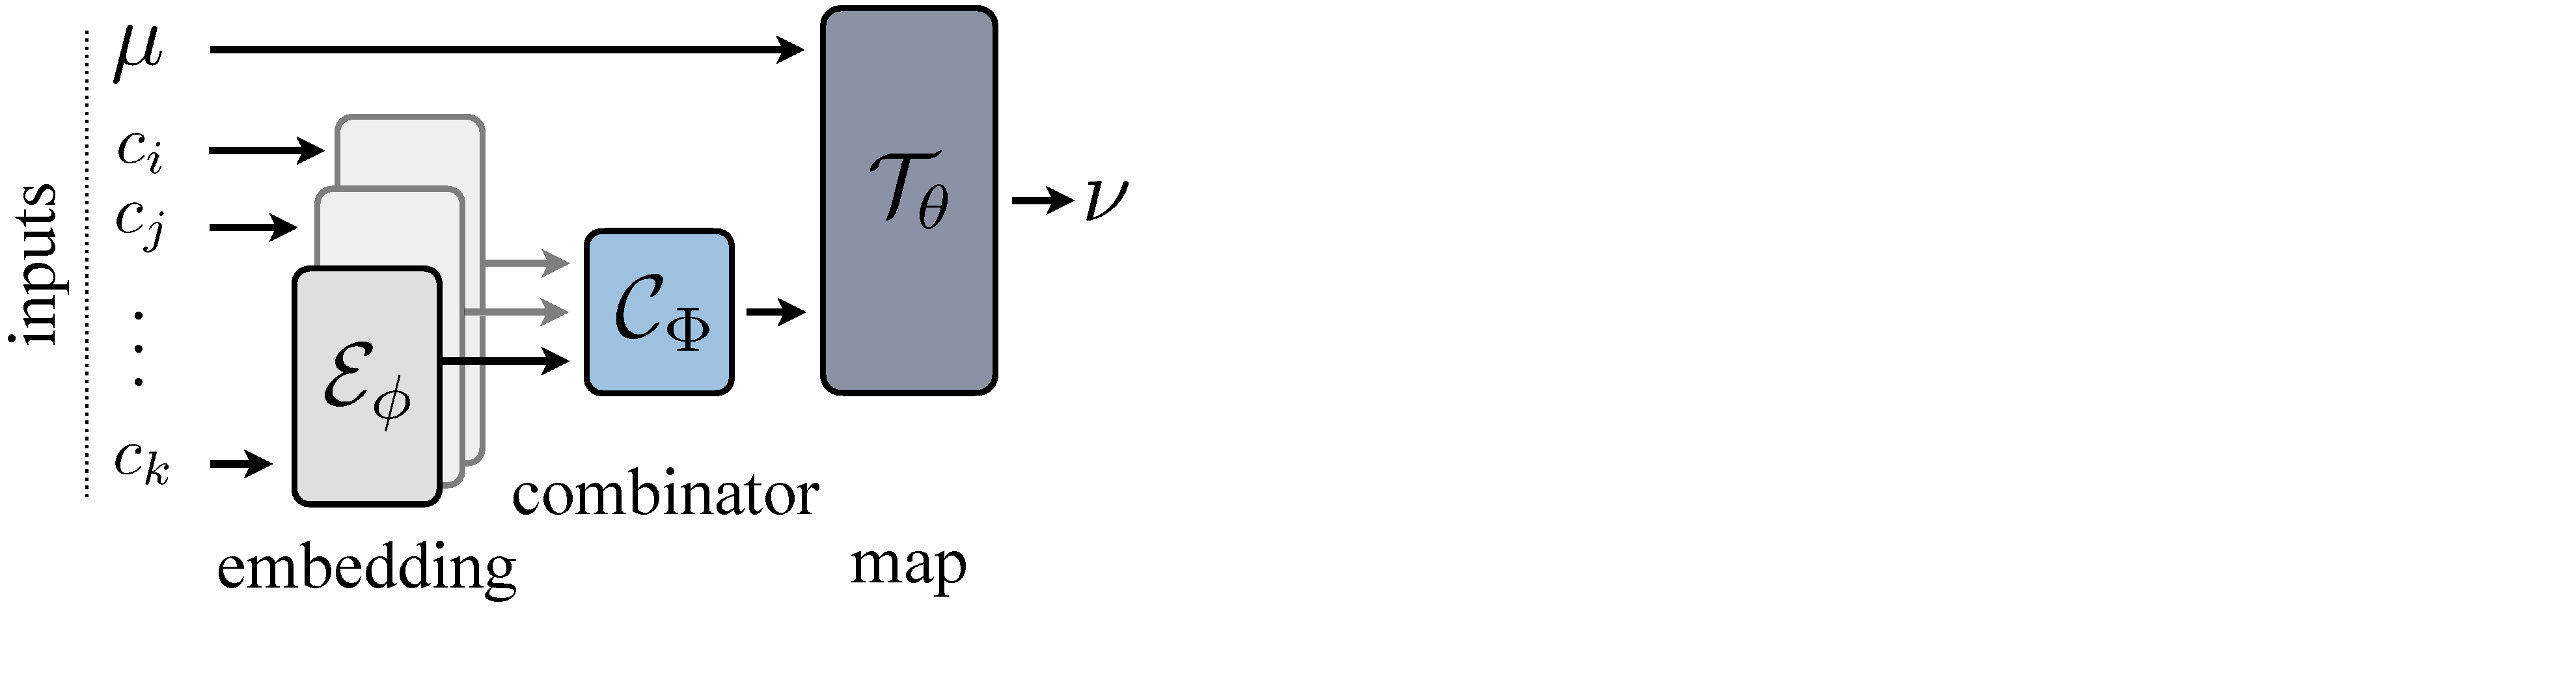
\includegraphics[width=0.4\textwidth]{figures/fig_architecture.pdf}
    \caption{\textbf{\textsc{CondOT} Architecture and Modules}. The embedding module $\mathcal{E}_\phi$ embeds arbitrary conditions $c$, which are then combined via module $\mathcal{C}_\Phi$. Using the processed contexts $c$, the map $\mathcal{T}_\theta(c)$ acts on $\mu$ to predict the target measure $\nu$. \vspace{-10pt}}
    \label{fig:architecture}
\end{wrapfigure}

\paragraph{Mode of action embedding $\mathcal{E}_\text{moa}$.}
In \textsc{CondOT}, we thus construct so-called \acrfull{MOA} embeddings, by computing an embedding $\mathcal{E}_\text{moa}$ that encourages actions $a$ with a similar effect on target population $\nu$ to have a similar representation.
Such mode-of-action embeddings map actions into a latent space based on their mechanism of action and effect on the target population.
In the fashion of word embeddings \citep{mikolov2013efficient, mikolov2013distributed, mikolov2013linguistic}, we require actions with similar effects to be closely embedded in the learned representation.
This means, however, that we require some sample access of target population particles, i.e., perturbed cells by individual compounds (not in combination).
While several metric embeddings are possible \citep{chopra2005learning}, we here test a simple multi-dimensional scaling-based embedding \citep{mead1992review}.
For this, we compute the pairwise Wasserstein distance matrix between all target populations of different individual perturbations. We then compute a 10-dimensional MDS embedding based on the stress minimization using a majorization algorithm (\texttt{smacof}) \citep{de2009multidimensional} of \texttt{sklearn} \citep{pedregosa2011scikit}, which serves as a descriptor for each individual perturbation.
In \cref{sec:evaluation_condot}, we analyze several embedding types for different use cases.

\subsubsection{Combinator Module $\mathcal{C}$}
\looseness -1 While we often have access to contexts $c$ in isolation, it is crucial to infer the effect of contexts applied in combination. A prominent example is cancer combination therapies, in which multiple treatment modalities are administered in combination to enhance treatment efficacy \citep{kummar2010utilizing}.
In these settings, the mode of operation between individual contexts $c$ is often not known, and can thus not be directly modeled via simple arithmetic operations such as 
\texttt{min, max, sum, mean}.
While we test as a baseline the case, applicable to one-hot-embeddings, where simple additions are used to model these combinations, we propose to augment the \textsc{CondOT} architecture with a parameterized combinator module $\mathcal{C}_\Phi$. We consider the following combinator modules:

\paragraph{Multi-hot combinator $\mathcal{C}^\text{ohe}_+$.}
A na\"ive way of constructing the combinator is to combine different actions via multi-hot encodings. If all single perturbations are observed during training, each individual action can be represented via a one-hot encoding. The potential combination of different actions is then encoded by adding the respective one-hot encodings, resulting in a multi-hot encoding for each combination.
A limitation of this embedding, however, is that it cannot generalize to unknown actions after training.

\paragraph{Deep set combinator $\mathcal{C}^\text{moa}_\Phi$.}
When not considering one-hot-based embeddings and when aiming to generalize to unseen perturbations, we need a combinator module that learns how to associate different individual embeddings with each other to receive a joint embedding.
As we, for now, do not make an assumption on the order of the perturbation, we consider a permutation-invariance network architecture such as deep sets \citep{zaheer2017deep} with parameters $\Phi$. Taking a set of arbitrary size $k$ containing individual context embeddings $\{\mathcal{E}_\text{moa}(c^1), \mathcal{E}_\text{moa}(c^2), \dots, \mathcal{E}_\text{moa}(c^k)\}$, it returns a learned combination embedding $\hat{c}_i = \mathcal{C}_\Phi(\mathcal{E}_\text{moa}(c^1), \mathcal{E}_\text{moa}(c^2), \dots, \mathcal{E}_\text{moa}(c^k))$.
% If interactions between the context variables exist, $\mathcal{C}_\Phi$ can be represented via classical message-passing network architectures~\citep{gilmer2020message,kipf2018neural}.
Receiving a flexible number of inputs from the embedding module $\mathcal{E}_\phi$, \textsc{CondOT} allows for joint training of the PICNN parameters $\theta$, embedding parameters $\phi$, and combinator parameters $\Phi$ in a single, end-to-end differentiable architecture.


\subsubsection{Training Procedure}

\looseness -1 Given a dataset $\mathcal{D}=\{c_i, (\mu_i, \nu_i) \}_{i=0}^N$ of $N$ pairs of populations before $\mu_i$ and after transport $\nu_i$ connected to a context $c_i$, we follow a similar strategy as introduced in \cref{sec:neural_solvers} to learn map $\mathcal{T}_\theta(c_i)$. 
The training loss aims at making sure the map $\mathcal{T}_\theta(c_i)$ is an OT map from $\mu_i$ to $\nu_i$, where $c_i$ may either be the original label itself or its embedded/combined formulation in more advanced tasks. To handle the Legendre transform in \eqref{eq:dual-cvx}, we use the proxy dual objective defined in \eqref{eq:ot-minmax} \citep{makkuva2020optimal} in place of \eqref{eq:dual-cvx} to minimize our overall loss~\eqref{eq:supdual}.

We then parameterize the potentials $\varphi$ and $g$ using two PICNNs, i.e., $\text{PICNN}_{\theta}$ and $\text{PICNN}_{\phi}$, that already integrate an embedding and/or combinator module. The regularization in \eqref{eq:ot-minmax} thereby promotes that for any $c$, $\text{PICNN}_{\phi}(\cdot,c)$ resembles the Legendre transform of the other network, i.e., $\text{PICNN}_{\theta^\star}(\cdot,c)$.
Parameters of all three modules are trained jointly through the alternate min-max optimization introduced in \eqref{eq:cellot-optim}, replacing the \acrshort{ICNN} architecture in loss functions \eqref{eq:makkuva_f_loss}-\eqref{eq:makkuva_g_loss} with \acrshortpl{PICNN}, i.e.,
\begin{align*} 
    \ell_\varphi(\mu, \nu, c; \theta) &= \mathbb{E}_{x \sim \mu}[\text{PICNN}_{\phi}(x, c)] - \mathbb{E}_{y \sim \nu}[\text{PICNN}_{\theta}(\nabla \text{PICNN}_{\phi}(y, c), c)], \\
    \ell_g(\mu, \nu, c; \phi) &= -\mathbb{E}_{y \sim \nu}[\langle y, \nabla \text{PICNN}_{\phi}(y, c)\rangle-\text{PICNN}_{\theta}(\nabla \text{PICNN}_{\phi}(y, c), c)].
\end{align*}
For more details, see \cref{sec:neural_solvers}.

\begin{table*}[t]
    \caption{Evaluation of drug effect predictions from control cells to cells treated with drug Givinostat when conditioning on various covariates influencing cellular responses such as drug dosage and cell type. Results are reported based on MMD and the $\ell_2$ distance between perturbation signatures of marker genes in the 1000-dimensional gene expression space.}
    \label{tab:exp_scalar_covariate_sciplex}
    \centering
\adjustbox{max width=\linewidth}{%
    \begin{tabular}{lccccc}
    \toprule
         \textbf{Method} & \multicolumn{5}{c}{\textbf{Conditioned on Drug Dosage}} \\
         & \multicolumn{2}{c}{In-Sample} && \multicolumn{2}{c}{Out-of-Sample}\\
         \cmidrule{2-3} \cmidrule{5-6}
         & MMD & $\ell_2(\text{PS})$ && MMD & $\ell_2(\text{PS})$ \\
    \midrule
        \textsc{CPA} \citep{lotfollahi2021compositional} & 0.1502 $\pm$ 0.0769 & 2.47 $\pm$ 2.89 && 0.1568 $\pm$ 0.0729 & 2.65 $\pm$ 2.75 \\
        \textsc{ICNN OT} \citep{makkuva2020optimal} & 0.0365 $\pm$ 0.0473 & 2.37 $\pm$ 2.15 && 0.0466 $\pm$ 0.0479 & 2.24 $\pm$ 2.39 \\
        \textsc{CondOT} (Identity initialization) & 0.0111 $\pm$ 0.0055 & 0.63 $\pm$ 0.09 && 0.0374 $\pm$ 0.0052 & 2.02 $\pm$ 0.10 \\
        \textsc{CondOT} (Gaussian initialization) & 0.0128 $\pm$ 0.0081 & 0.60 $\pm$ 0.11 && 0.0325 $\pm$ 0.0062 & 1.84 $\pm$ 0.14 \\
    \bottomrule  \\
    \end{tabular}
}
	\raggedright
\adjustbox{max width=.66\linewidth}{%
	\begin{tabular}{lcccccccc}
    \toprule
         \textbf{Method} & \multicolumn{2}{c}{\textbf{Conditioned on Cell Line}} \\
         & \multicolumn{2}{c}{In-Sample} \\
         \cmidrule{2-3}
         & MMD & $\ell_2(\text{PS})$ \\
    \midrule
        \textsc{CPA} \citep{lotfollahi2021compositional} & 0.2551 $\pm$ 0.006 & 2.71 $\pm$ 1.51 \\
        \textsc{ICNN OT} \citep{makkuva2020optimal} & 0.0206 $\pm$ 0.0109 & 1.16 $\pm$ 0.75 \\
        \textsc{CondOT} (Identity initialization) & 0.0148 $\pm$ 0.0078 & 0.39 $\pm$ 0.06 \\
        \textsc{CondOT} (Gaussian initialization) & 0.0146 $\pm$ 0.0074 & 0.41 $\pm$ 0.07 \\
    \bottomrule
    \end{tabular}
}
\end{table*}

\begin{figure*}
    \centering
    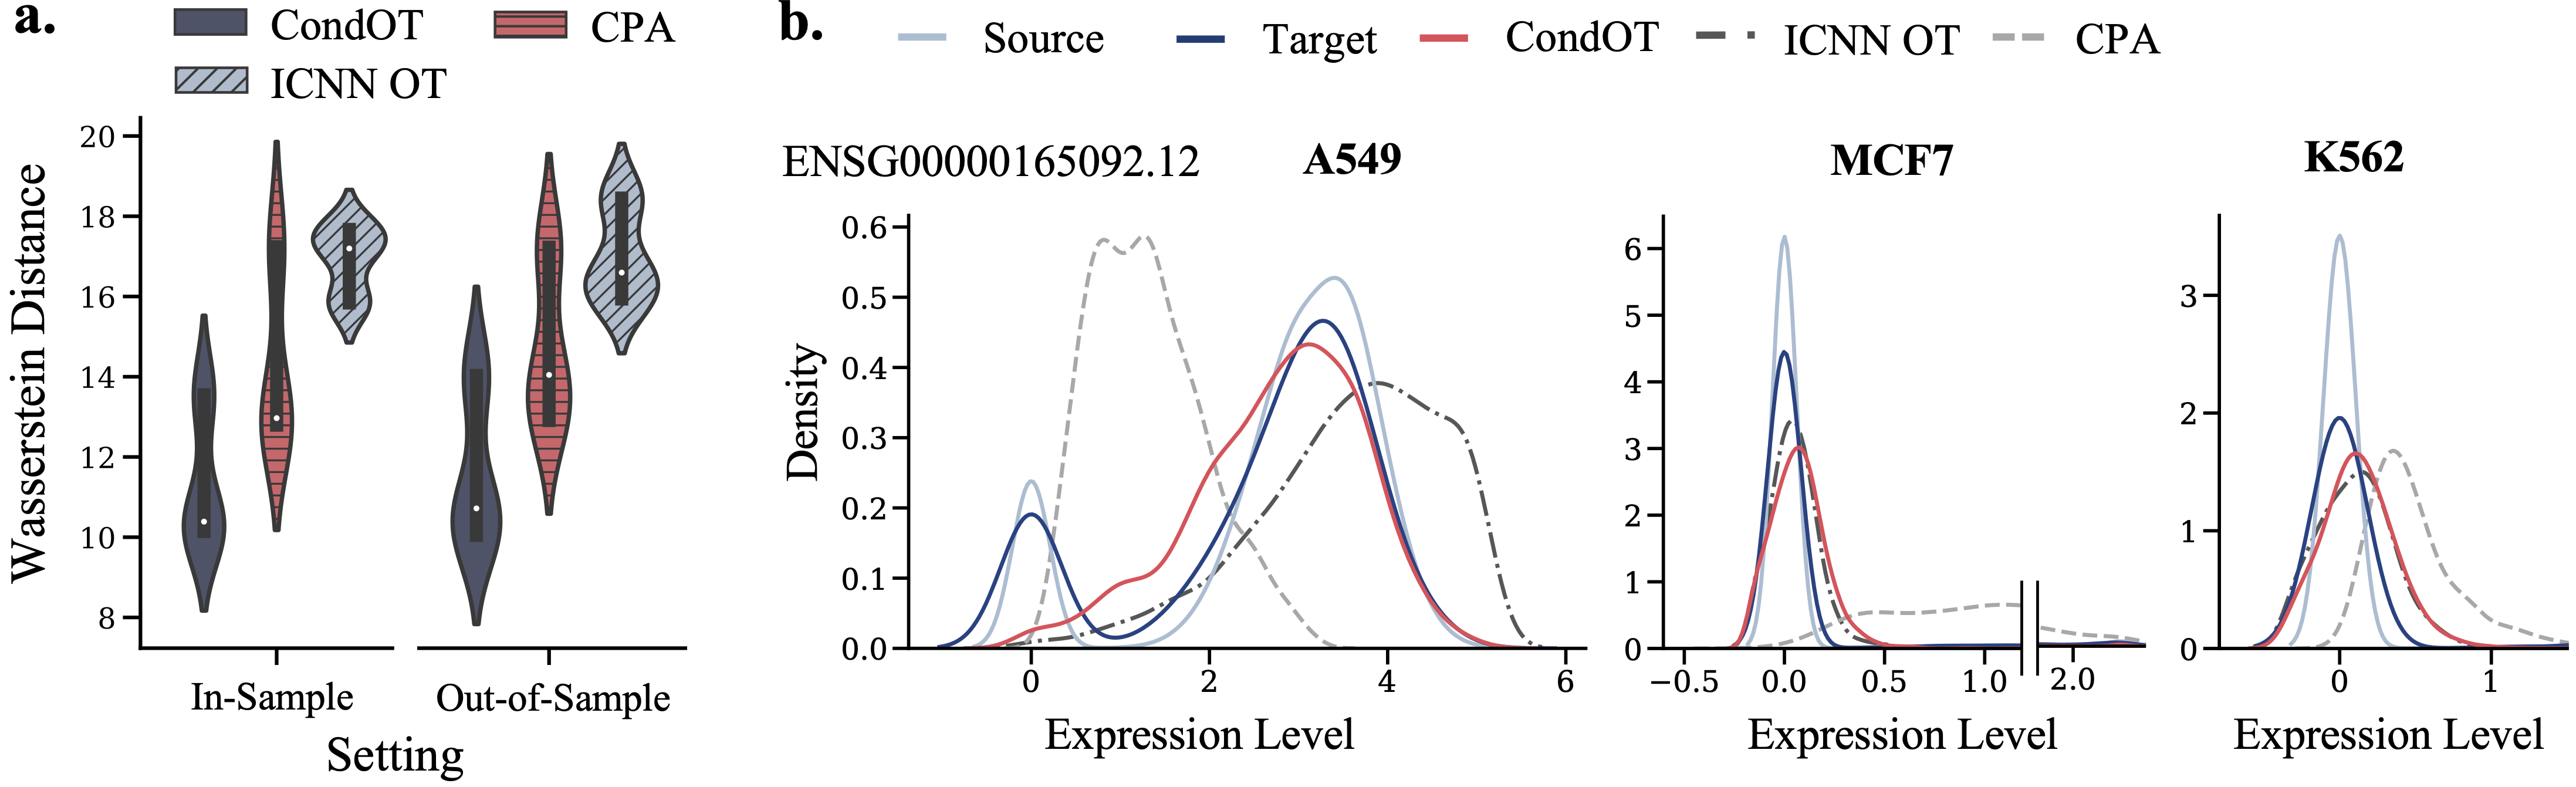
\includegraphics[width=\textwidth]{figures/fig_sciplex_main_results.png}
    \caption{\textbf{a.} \looseness -1 Predictive performance of \textsc{CondOT} and baselines w.r.t. the entropy-regularized Wasserstein distance on drug dosages \emph{in-sample}, i.e., seen during training, and \emph{out-of-sample}, i.e., unseen during training. \textbf{b.} Marginal distributions of observed source and target distributions, as well as predictions on perturbed distributions by \textsc{CondOT} and baselines of an exemplary gene across different cell lines. The predicted marginals of each method should match the marginal of the target population.}
    \label{fig:exp_scalar_sciplex}
\end{figure*}

\section{Empirical Evaluation} \label{sec:evaluation_condot}

\looseness -1 Biological cells undergo changes in their molecular profiles upon chemical, genetic, or mechanical perturbations. These changes can be measured using recent technological advancements in high-resolution multivariate single-cell biology. Measuring single cells in their unperturbed or perturbed state requires, however, destroying them, resulting in populations $\mu$ and $\nu$ that are unpaired. The relevance of OT to that comes from its ability to resolve such ambiguities through OT maps, 
% which can provide more general functions that can predict molecular responses, 
holding promises of a better understanding of health and disease. 
We consider various high-dimensional problems arising from this scenario to evaluate the performance of \textsc{CondOT} versus other baselines.
% Here we assume that  capture that cells at any time are drawn from a probability distribution in gene-expression space.

\subsection{Modeling Dosage-Sensitive Treatment Responses to Cancer Drugs} \label{sec:eval_scalar}

% The evolution of single-cell populations during a developmental process can be monitored by sampling, every now and then, representative cells of the system, and measuring their gene expression features in order to trace the differentiation across multiple snapshots.
% Inferring a matching of ancestor to descendant fates is a crucial step toward a better understanding of the molecular programs that guide cell differentiation of these evolutionary processes.

% In the following, we apply \textsc{CondOT} to embryoid body single-cell RNA sequencing (scRNA-seq) data \citep{moon2019}, describing the differentiation of human embryonic stem cells grown as embryoid bodies into diverse cell lineages over a period of 27 days.
% We aim at infering the transport map $T_\theta(\delta t)$ which predicts the development of a cell population at time $t_i$ into cell states at time $t_{i+1}$, i.e., $T_\theta(\delta t)_\sharp \mu_{i} = \mu_{i+1}$, where $\delta t = t_{i+1} - t_{i}$.
% We learn $T_\theta$ by utilizing \citeauthor{brenier1987decomposition}'s theorem and parameterizing $T_\theta = \nabla \text{PICNN}_\theta$ taking as input the measure at the previous time point $\mu_{i}$ as well as the time interval $\delta t$ during which the cells are expected to evolve (see \cref{sec:neural_primal} for more details).
% We compare our method to classical forward Euler schemes, previously proposed to learn time-varying single-cell dynamics \citep{hashimoto2016learning, bunne2022proximal}.

% Small molecular drugs can have profound effects on the cellular phenotype by altering signaling cascades and other molecular programs.
\looseness -1 Upon application of a molecular drug, the state of each cell $x_i$ of the unperturbed population is altered, and observed in population $\nu$.
Molecular drugs are often applied at different dosage levels $t$, and the magnitude of changes in the gene expression profiles of single cells highly correlates with that dosage. 
We seek to learn a global, parameterized transport map $\mathcal{T}_\theta$ sensitive to that dosage.% and accurately describe perturbed cellular states at different dosage levels.
We evaluate our method on the task of inferring single-cell perturbation responses to the cancer drug Givinostat, a histone deacetylase inhibitor with potential anti-inflammatory, anti-angiogenic, and antineoplastic activities \citep{srivatsan2020massively}, applied at different dosage levels, i.e., $t \in \{10\,$nM, $100\,$nM, $1,000\,$nM, $10,000\,$nM$\}$. The dataset contains $3,541$ cells described with the gene expression levels of $1,000$ highly-variable genes.
In a first experiment, we measure how well \textsc{CondOT} captures the drug effects at different dosage levels via distributional distances such as MMD~\citep{gretton2012kernel} and the $\ell_2$-norm between the corresponding \acrfull{PS}, as well as the entropy-regularized Wasserstein distance~\citep{cuturi2013sinkhorn}. We compute the metrics on 50 marker genes, i.e., genes mostly affected upon perturbation.
To put \textsc{CondOT}'s performance into perspective, we compare it to current state-of-the-art baselines~\citep{lotfollahi2021compositional} as well as parameterized Monge maps without context variables \citep[\textsc{ICNN OT}]{bunne2021learning, makkuva2020optimal}.
As visible in Table~\ref{tab:exp_scalar_covariate_sciplex} and \cref{fig:exp_scalar_sciplex}a, \textsc{CondOT} achieves consistently more accurate predictions of the target cell populations at different dosage levels than OT approaches that cannot utilize context information, demonstrated through a lower average loss and a smaller variance.
This becomes even more evident when moving to the setting where the population has been trained only on a subset of dosages and we test \textsc{CondOT} on \emph{out-of-sample} dosages. Table~\ref{tab:exp_scalar_covariate_sciplex} and \cref{fig:exp_scalar_sciplex}a demonstrate that \textsc{CondOT} is able to generalize to previously \emph{unknown} dosages, thus learning to interpolate the perturbation effects from dosages seen during training.
% We further provide an additional comparison of \textsc{CondOT}, operating in the multi-task setting, to the single-task performance of optimal transport-based methods \cref{app:add_baseline}. While the single-task setting of course fails to generalize to new contexts and requires all contexts to be distinctly known, it provides us with a \textit{pseudo} lower bound, which \textsc{CondOT} is able to reach (see Table~\ref{tab:lower_bound}).
% For dosages, we build a dosage encoder module $\mathcal{E}_\text{dosage}$ which can integrate known dosage-response curves (e.g., linear, sigmoid, or more complex relationships). ...

\begin{figure*}[t]
    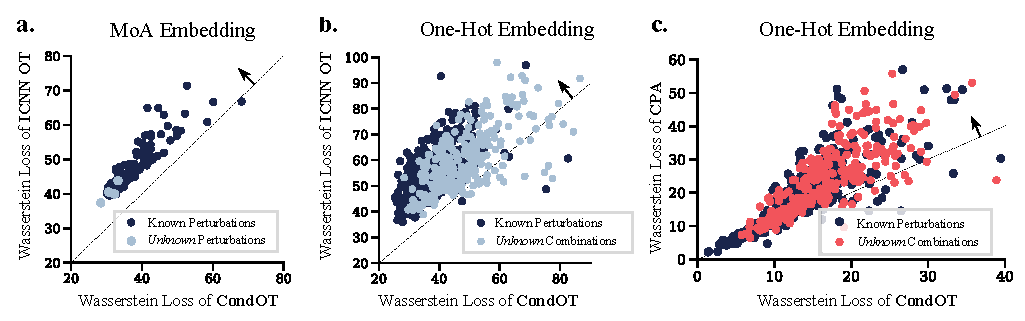
\includegraphics[width=\textwidth]{figures/fig_action_comb_comparison_scatter.pdf}
    \caption{Comparison between \textbf{a.} \textsc{CondOT} and \textsc{ICNN OT}~\citep{makkuva2020optimal} based on embedding $\mathcal{E}_\text{moa}$ \textbf{b.} as well as $\mathcal{E}_\text{ohe}$, and \textbf{c.} \textsc{CondOT} and \textsc{CPA}~\citep{lotfollahi2021compositional} based on embedding $\mathcal{E}_\text{ohe}$ on \emph{known} and \emph{unknown} perturbations or combinations. Results above the diagonal suggest the higher predictive performance of \textsc{CondOT}.}
    \label{fig:exp_action_norman_scatter}
\end{figure*}


\subsection{Predicting Cell Type-Specific Treatment Responses to Cancer Drugs} \label{sec:eval_covariate}

\looseness -1 Molecular processes are often highly dependent on additional covariates that steer experimental conditions, and which are not present in the features measures in population $\mu$ or $\nu$.
This can be, for instance, factors such as different cell types clustered within the populations.
When the model can only be conditioned w.r.t. a small and \textit{fixed} set of metadata information, such as cell types, it is sufficient to encode these contexts using a one-hot encoding module $\mathcal{E}_\text{ohe}$.
To illustrate this problem, we consider cell populations comprising three different cell lines (A549, MCF7, and K562). As visible in Table~\ref{tab:exp_scalar_covariate_sciplex}, \textsc{CondOT} outperforms current baselines which equally condition on covariate information such as \textsc{CPA}~\citep{lotfollahi2021compositional}, assessed through various evaluation metrics.
Figure~\ref{fig:exp_scalar_sciplex}b displays a gene showing highly various responses towards the drug Givinostat dependent on the cell line. \textsc{CondOT} captures the distribution shift from control to target populations consistently across different cell lines.

\subsection{Inferring Genetic Perturbation Responses}

\looseness -1 To recommend personalized medical procedures for patients, or to improve our understanding of genetic circuits, it is key to be able to predict the outcomes of novel perturbations, arising from combinations of drugs or genetic perturbations. 
Rather than learning individual maps $T_\theta^a$ predicting the effect of individual treatments, we aim at learning a global map  $\mathcal{T}_\theta$ which, given as input the unperturbed population $\mu$ as well as the action $a$ of interest, predicts the cell state perturbed by $a$.
Thanks to its modularity, \textsc{CondOT} can not only learn a map $T_\theta$ for all actions \emph{known} during training but also generalize to \emph{unknown} actions, as well as potential \emph{combinations} of actions. We will discuss all three scenarios below.

\subsubsection{\textit{Known} Actions}
\label{sec:eval_action_known}

\looseness -1 In the following, we analyze \textsc{CondOT}'s ability to accurately predict phenotypes of genetic perturbations based on single-cell RNA-sequencing pooled \acrfull{CRISPR} screens \citep{norman2019exploring, dixit2016perturb}, comprising $98,419$ single-cell gene expression profiles with $92$ different genetic perturbations, each cell measured via a $1,500$ highly-variable gene expression vector.
As, in the first step, we do not aim at generalizing beyond perturbations encountered during training, we utilize again a one-hot encoding $\mathcal{E}_\text{ohe}$ to condition $\mathcal{T}_\theta$ on each perturbation $a$.
We compare our method to other baselines capable of modeling effects of a large set of perturbations such as \textsc{CPA} \citep{lotfollahi2021compositional}.
Often, the effect of genetic perturbations is subtle in the high-dimensional gene expression profile of single cells. Using ICNN-parameterized OT maps without context information, we can thus assess the gain in accuracy of predicting the perturbed target population by incorporating context awareness over simply predicting an average perturbation effect. 
Figure~\ref{fig:exp_action_norman_scatter}a and b demonstrate that compared to OT ablation studies, \cref{fig:exp_action_norman_scatter}c and \cref{fig:exp_action_norman_line}a for the current state-of-the-art method \textsc{CPA}~\citep{lotfollahi2021compositional}. Compared to both, \textsc{CondOT} captures the perturbation responses more accurately w.r.t. the Wasserstein distance.

\begin{figure*}[t]
    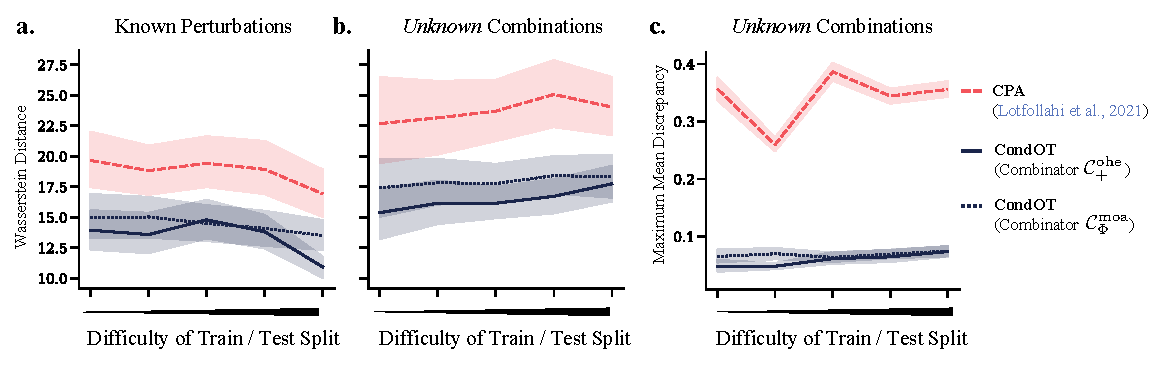
\includegraphics[width=1.1\textwidth]{figures/fig_action_comb_comparison_metrics.pdf}
    \caption{Predictive performance for \textbf{a.} known perturbations, \textbf{b.} unknown perturbations in combination w.r.t. regularized Wasserstein distance and \textbf{c.} MMD over different train/test splits of increasing difficulty for baseline \textsc{CPA} as well as \textsc{CondOT} with different combinators $\mathcal{C}^\text{ohe}_+$ and $\mathcal{C}^\text{moa}_\Phi$.}
    \label{fig:exp_action_norman_line}
\end{figure*}


\subsubsection{\textit{Unknown} Actions}
\label{sec:eval_action_unknown}

\looseness -1 With the emergence of new perturbations or drugs, we aim at inferring cellular responses to settings not explored during training.
One-hot encodings, however, do not allow us to model \emph{unknown} perturbations. 
This requires us to use an embedding $\mathcal{E}$, which can provide us with a representation of an unknown action $a^\prime$.
As genetic perturbations further have no meaningful embeddings as, for example, molecular fingerprints for drugs, we resort to mode-of-action embeddings introduced in \cref{subsec:combin}. Assuming marginal sample access to all individual perturbations, we compute a \acrfull{MDS}-based embedding from pairwise Wasserstein distances between individual target populations, such that perturbations with similar effects are closely represented. 
As current state-of-the-art methods are restricted to modeling perturbations via one-hot encodings, we compare our method to \textsc{ICNN OT} only. As displayed in \cref{fig:exp_action_norman_scatter}a, \textsc{CondOT} accurately captures the response of \emph{unknown} actions (BAK1, FOXF1, MAP2K6, MAP4K3), which were not seen during training, at a similar Wasserstein loss as perturbation effects seen during training.
 
 \begin{figure*}
    \centering
    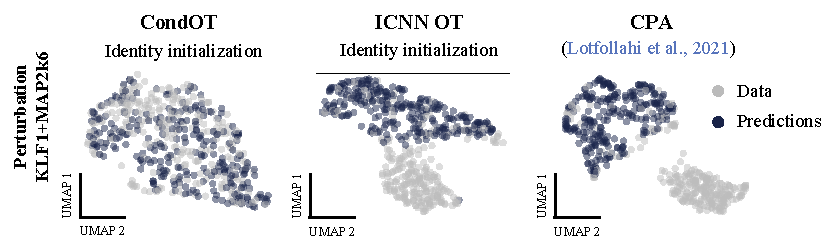
\includegraphics[width=0.9\textwidth]{figures/fig_action_comb_comparison_umap.pdf}
    \caption{\looseness -1 \acrshort{UMAP} embeddings of cells perturbed by the combination KLF1+MAP2K6 (gray) and predictions of \textsc{CondOT} (ours), \textsc{ICNN OT}~\citep{makkuva2020optimal}, and \textsc{CPA} (blue). While \textsc{CondOT} aligns well with observed perturbed cells, the baselines fail to capture subpopulations.}
    \label{fig:action_comb_comparison_umap}
\end{figure*}
 

\subsubsection{Actions in Combination}
\label{sec:eval_action_comb}

\looseness -1 While experimental studies can often measure perturbation effects in biological systems in isolation, the combinatorial space of perturbations in composition is too large to capture experimentally. Often, however, combination therapies are cornerstones of cancer therapy \citep{mokhtari2017combination}.
In the following, we test different combinator architectures to predict genetic perturbations in combination with single targets.
Similarly to \citet{lotfollahi2021compositional}, we can embed combinations by adding individual one-hot encodings of single perturbations (i.e., $\mathcal{C}^\text{ohe}_+$). In addition, we parameterize a combinator via a permutation-invariant deep set, as introduced in \cref{subsec:combin}, based on mode-of-action embeddings of individual perturbations (i.e., $\mathcal{C}^\text{moa}_\Phi$). 
We split the dataset into train/test splits of increasing difficulty: Initially containing all individual perturbations as well as some combinations, the number of perturbations seen in combination during training decreases over each split.
We compare different combinators to \textsc{ICNN OT} (\cref{fig:exp_action_norman_scatter}b) and \textsc{CPA}~\citep{lotfollahi2021compositional} (\cref{fig:exp_action_norman_scatter}c, \cref{fig:exp_action_norman_line}b, c). While the performance drops compared to inference on \emph{known} perturbations (\cref{fig:exp_action_norman_line}a) and decreases with increasing difficulty of the train/test split, \textsc{CondOT} outperforms all baselines.
When embedding these high-dimensional populations in a low-dimensional \acrshort{UMAP} space~\citep{umap}, one can see that \textsc{CondOT} captures the entire perturbed population, while \textsc{ICNN OT} and \textsc{CPA} fail in capturing certain subpopulations in the perturbed state (see \cref{fig:action_comb_comparison_umap}).


\section{Discussion}
We have developed the \textsc{CondOT} framework that is able to infer OT maps from not only one pair of measures but many pairs that come labeled with a context value. To ensure that \textsc{CondOT} encodes optimal transports, we parameterize it as a PICNN, an input-convex NN that modulates the values of its weights matrices according to a sequence of feature representations of that context vector. We showcased the generalization abilities of \textsc{CondOT} in the extremely challenging task of predicting outcomes for unseen combinations of treatments. These abilities and PICNN more generally hold several promises, both as an augmentation of the \texttt{OTT} toolbox~\citep{cuturi2022optimal} and for future applications of OT to single-cell genomics.
